% Author: Izaak Neutelings (May 2018)
% Inspiration: https://tex.stackexchange.com/questions/113900/draw-polarized-light
\documentclass[border=10pt,tikz]{standalone}
\usepackage{amsmath} % for \text
\usepackage{tikz}
\usepackage{physics}
\tikzset{>=latex} % for LaTeX arrow head
\usepackage{xcolor}
\usepackage{amsmath}
\colorlet{myblue}{black!40!blue}
\colorlet{myred}{black!40!red}
\colorlet{vcol}{green!50!black}
\colorlet{Ecol}{orange!90!black}
\colorlet{EVcol}{orange!80!black!60}
\colorlet{Bcol}{violet!90}
\begin{document}

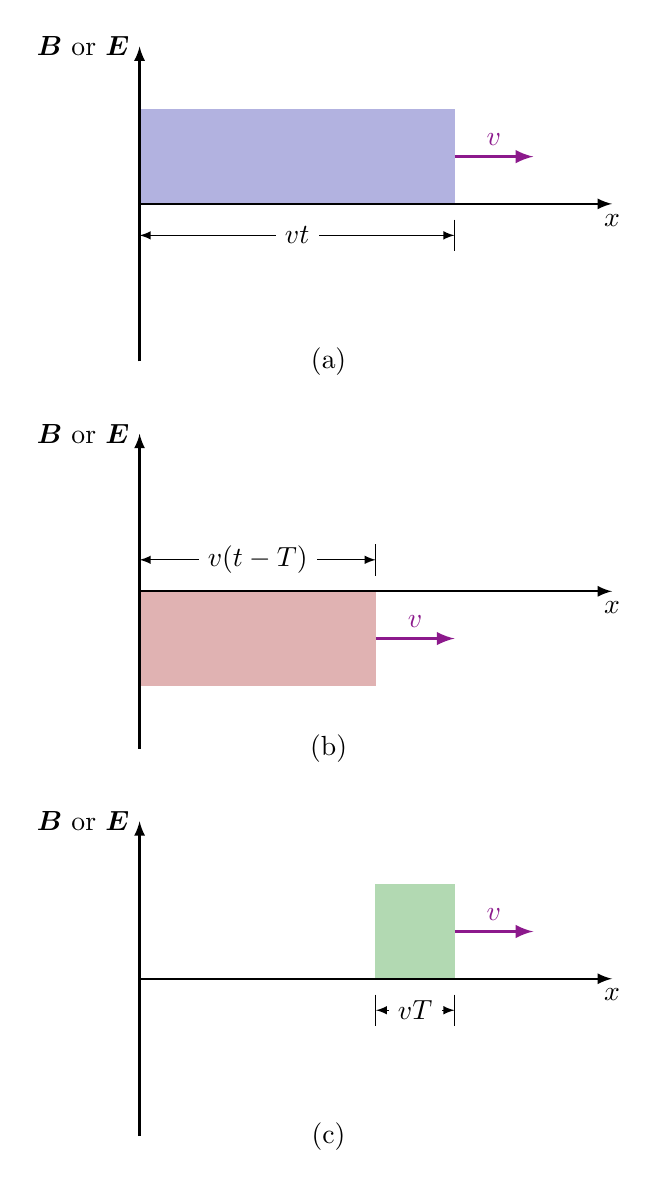
\begin{tikzpicture}[scale=2]
    \begin{scope}
        \filldraw[myblue!30] (0, 0) rectangle (2, 0.6);
        \draw[thick, ->] (0, 0) -- (3, 0) node [below] {$x$};
        \draw[thick, ->] (0, -1) -- (0, 1) node [left] {$\boldsymbol{B}$ or $\boldsymbol{E}$};
        \draw[] (2, -0.1) -- (2, -0.3);
        \draw[<->] (0, -0.2) -- (2, -0.2) node[midway, fill=white] {$vt$};
        \node[] at (1.2, -1) {(a)};
        \draw[color=Bcol, very thick, ->] (2, 0.3) -- (2.5, 0.3) node[midway, above]{$v$};
    \end{scope}

    \begin{scope}[yshift=-70]
        \filldraw[myred!30] (0, -0.6) rectangle (1.5, 0);
        \draw[thick, ->] (0, 0) -- (3, 0) node [below] {$x$};
        \draw[thick, ->] (0, -1) -- (0, 1) node [left] {$\boldsymbol{B}$ or $\boldsymbol{E}$};
        \draw[] (1.5, 0.1) -- (1.5, 0.3);
        \draw[<->] (0, 0.2) -- (1.5, 0.2) node[midway, fill=white] {$v(t-T)$};
        \node[] at (1.2, -1) {(b)};
        \draw[color=Bcol, very thick, ->] (1.5, -0.3) -- (2, -0.3) node[midway, above]{$v$};
    \end{scope}

    \begin{scope}[yshift=-140]
        \filldraw[vcol!30] (1.5, 0) rectangle (2, 0.6);
        \draw[thick, ->] (0, 0) -- (3, 0) node [below] {$x$};
        \draw[thick, ->] (0, -1) -- (0, 1) node [left] {$\boldsymbol{B}$ or $\boldsymbol{E}$};
        \draw[] (1.5, -0.1) -- (1.5, -0.3);
        \draw[] (2, -0.1) -- (2, -0.3);
        \draw[<->] (1.5, -0.2) -- (2, -0.2) node[midway, fill=white] {$vT$};
        \node[] at (1.2, -1) {(c)};
        \draw[color=Bcol, very thick, ->] (2, 0.3) -- (2.5, 0.3) node[midway, above]{$v$};
    \end{scope}

\end{tikzpicture}
\end{document}